%! Author = Philipp Emmenegger
%! Date = 09/06/2021

\section{Design Patterns}
\begin{itemize}
    \item Stories of repeatedly successful engineering
    \item Explaining the context and/or problem
    \item Describing a generic solution
    \item Mentoring viable alternatives
    \item Listing benefits and drawbacks
\end{itemize}
\textit{Design patterns are...}
\begin{itemize}
    \item Discoveries not inventions
    \item an efficient vocabulary
    \item describing a generic solution with "roles"
    \item honest
\end{itemize}
\textit{Are not...}
\begin{itemize}
    \item ready to use
    \item a golden hammer for every problem
    \item replacements for design principles
    \item replacements for software architecture
\end{itemize}

\subsection{Patterns vs. Principles}
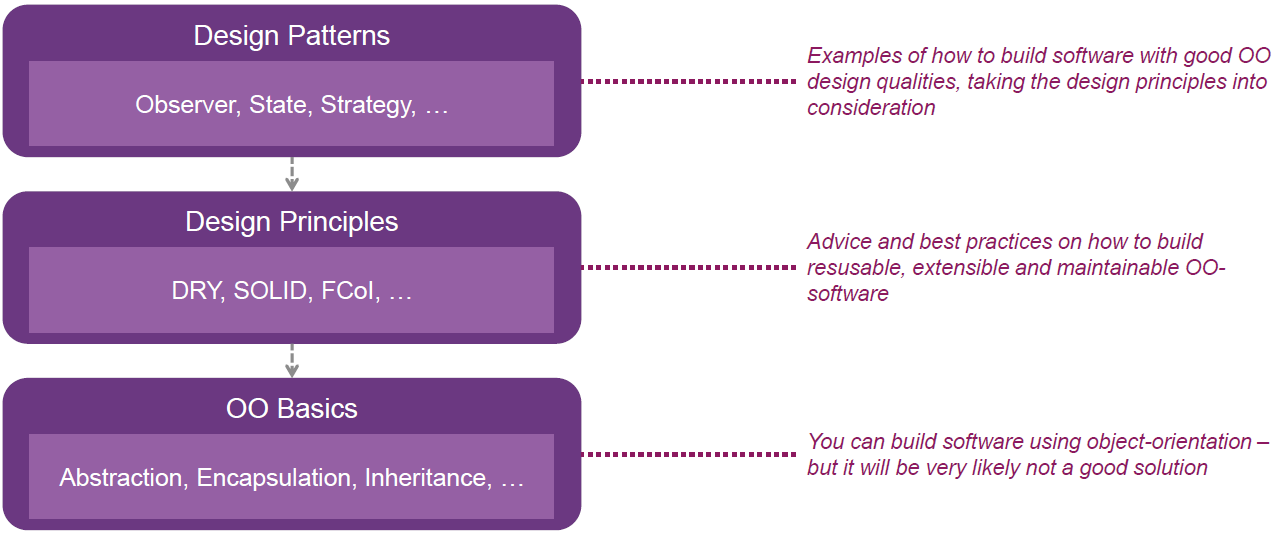
\includegraphics[width=\linewidth]{../img/patterns_vs_principles.png}

\subsection{GoF Design patterns}
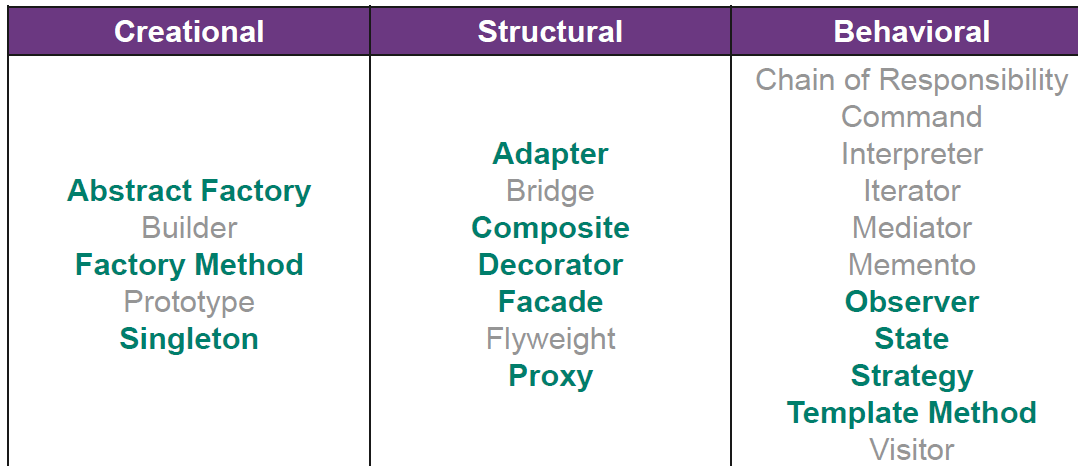
\includegraphics[width=\linewidth]{../img/gof_design_patterns.png}

\subsection{MVC, MVP, MVVM}
\begin{itemize}
    \item Design patterns dealing with presentation
    \item Not from the GoF book
    \item Very often compound from GoF-patterns
    \begin{itemize}
        \item Composite: to build a control-hierarchy
        \item Observer: to inform V about changes
        \item Strategy: to decouple V from C/P
    \end{itemize}
\end{itemize}

\subsection{Observer}
Define a one-to-many dependency between objects so that when one object changes state, all its dependents are notified and updated automatically.\\
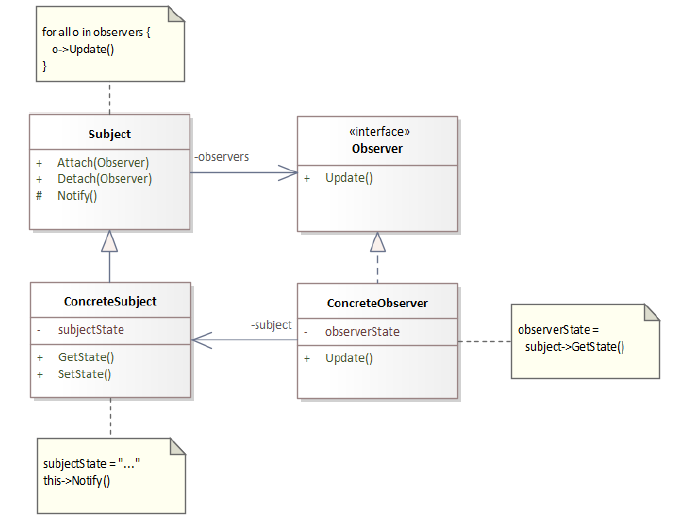
\includegraphics[width=0.85\linewidth]{../img/observer_pattern.png}

\subsection{State}
Allow an object to alter its behaviour when its internal state changes. The object will appear to change its class.
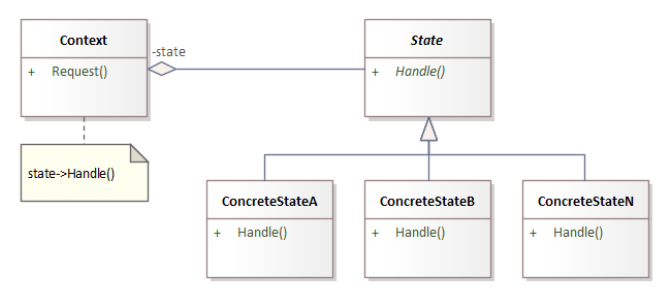
\includegraphics[width=0.85\linewidth]{../img/state_pattern.png}
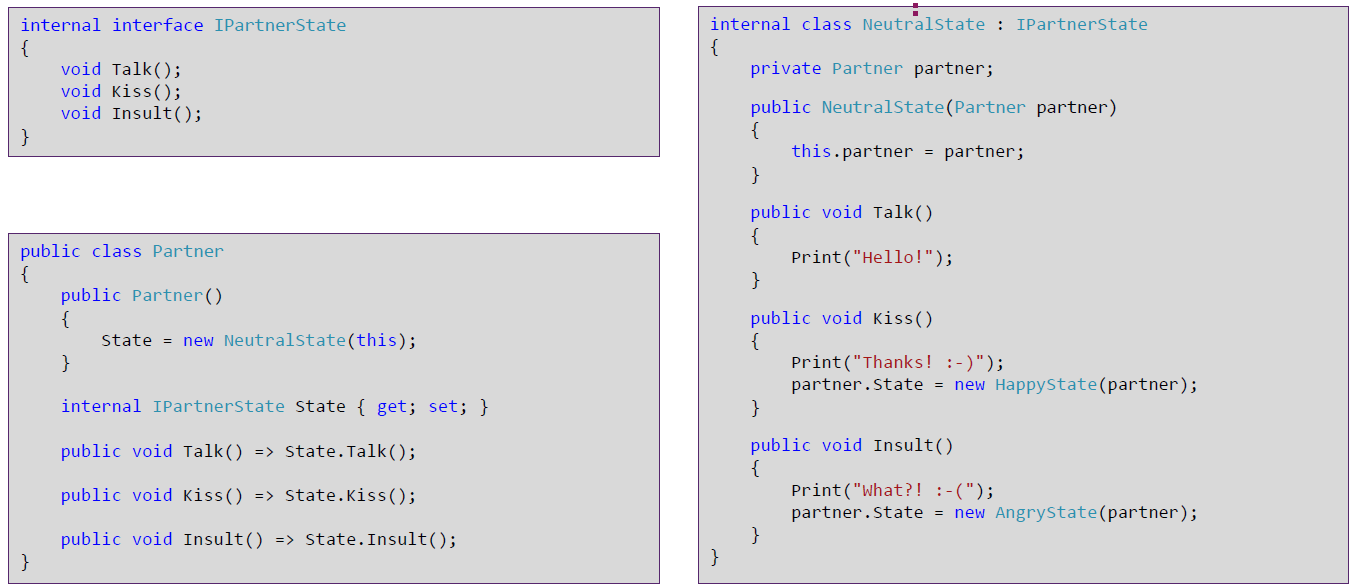
\includegraphics[width=\linewidth]{../img/state_pattern_code.png}

\subsection{Strategy}
Define a family of algorithms, encapsulate each one and make them interchangeable.\\
Strategy lets the algorithm vary independently from clients that use it.\\
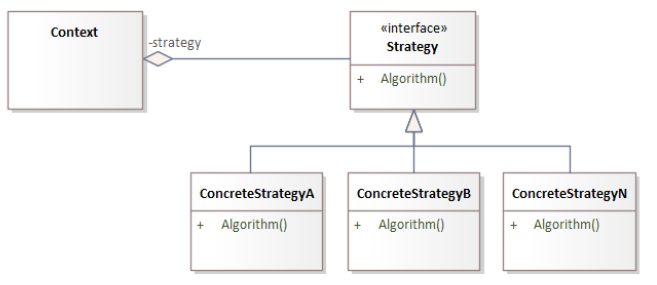
\includegraphics[width=0.85\linewidth]{../img/strategy_pattern.png}
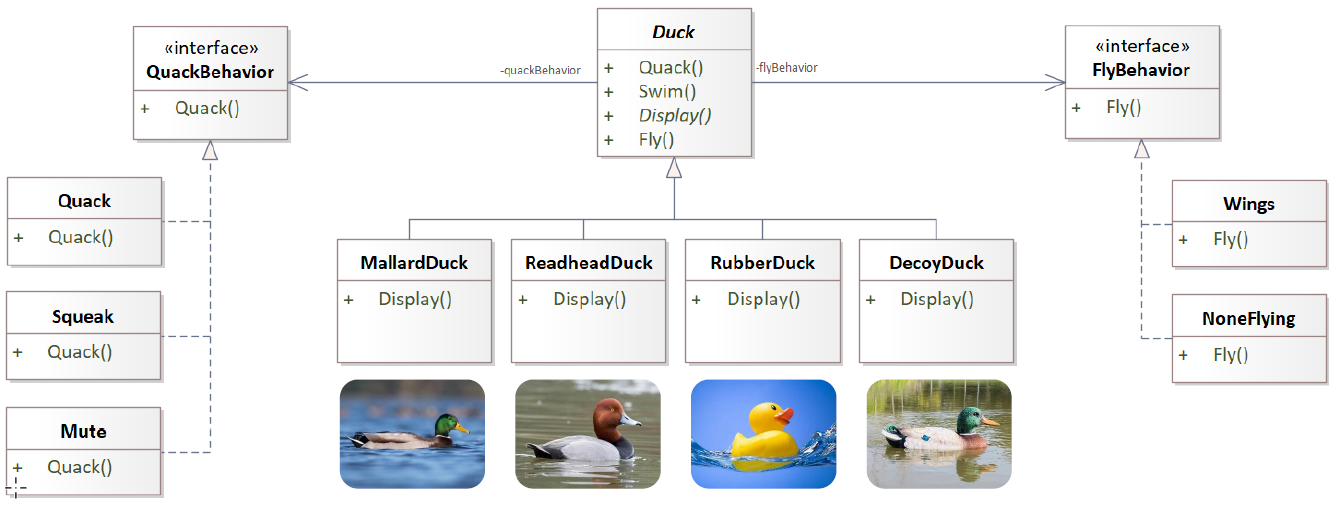
\includegraphics[width=\linewidth]{../img/strategy_pattern_duck_pond.png}
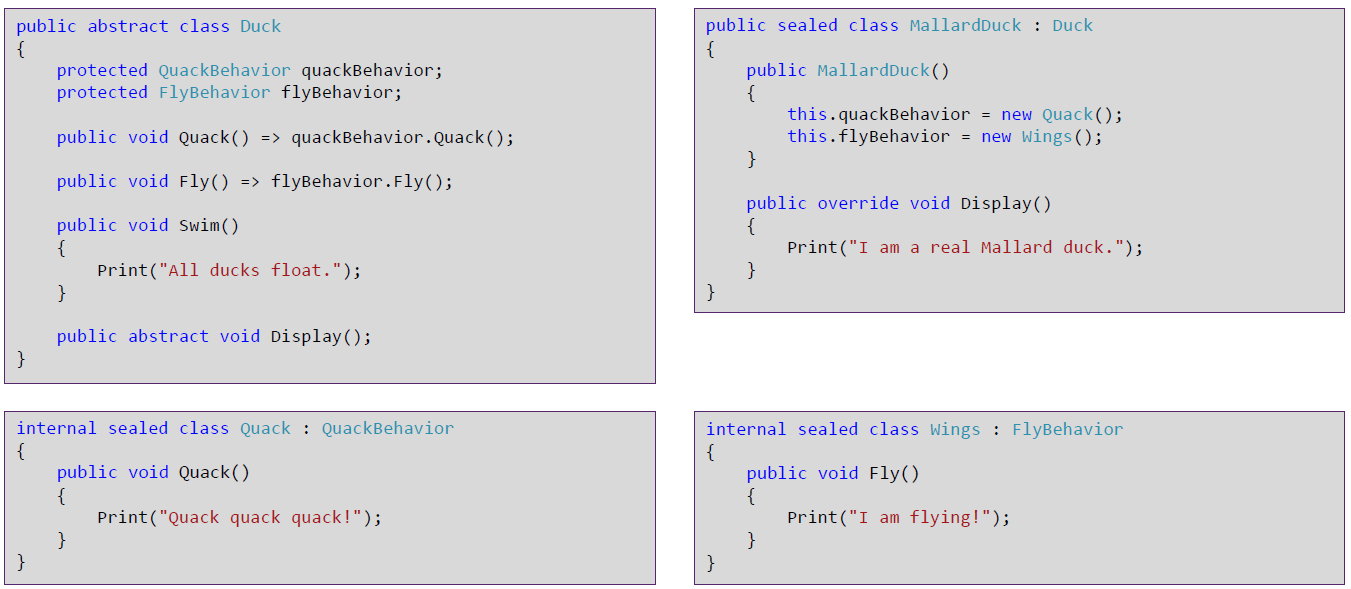
\includegraphics[width=\linewidth]{../img/strategy_pattern_code.png}

\subsubsection{NULL-Objects}
\begin{itemize}
    \item Classes implementing an interface wih empty methods
    \item Mute / NoneFlying in Duck Game
    \item Useful to get rid of null-checks and the risk of NullPointerException
\end{itemize}

\subsubsection{Dependency Injection}
\begin{itemize}
    \item Possible to get rid of all subtypes and inject the full behaviour using the constructor
    \item Constructor injection
\end{itemize}
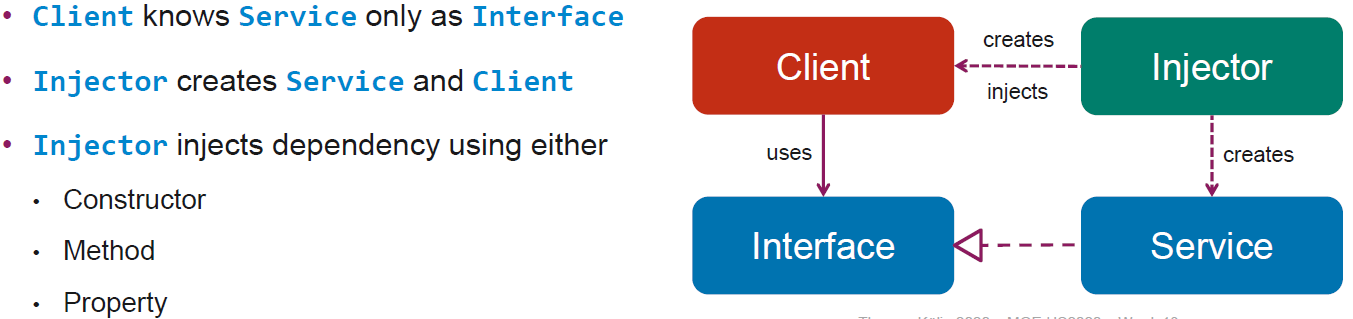
\includegraphics[width=\linewidth]{../img/strategy_pattern_DI.png}

\subsection{Strategy vs. State}
\textbf{State Pattern}
\begin{itemize}
    \item Encapsulates state behaviour
    \item Context hides internal state transitions
    \item Context switches its visible behaviour
    \item Replaces conditionals with compositions
\end{itemize}
\textbf{Strategy Pattern}
\begin{itemize}
    \item Encapsulates algorithmic behaviour
    \item Clients can configure Context with strategy
    \item Context mostly remains its visible behaviour
    \item Replaces inheritance with composition
\end{itemize}

\subsection{Template Method}
Define the skeleton of an algorithm in an operation, deferring some steps to subclasses.\\
Template Method lets subclasses redefine certain steps of an algorithm without changing the algorithm's structure.\\
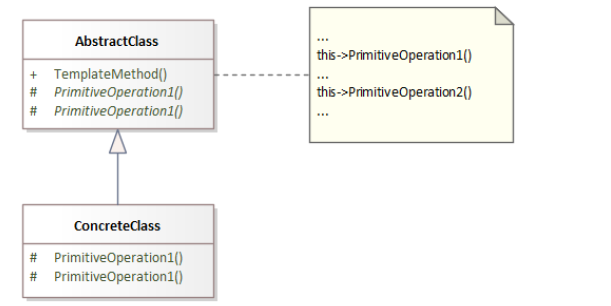
\includegraphics[width=0.7\linewidth]{../img/template_method.png}\\
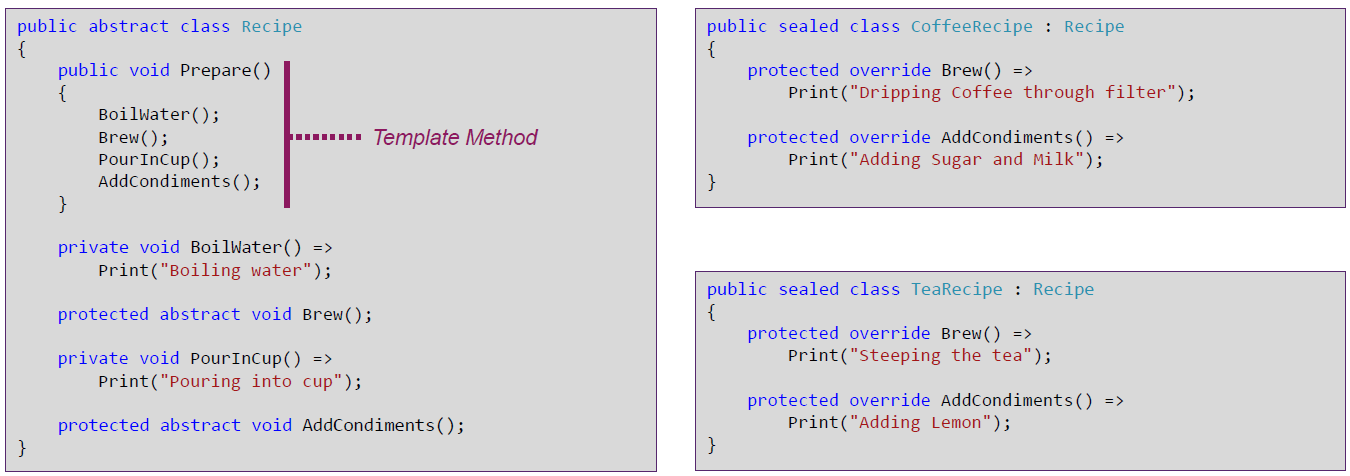
\includegraphics[width=\linewidth]{../img/template_method_code.png}



























